\subsection{Quotients of spheres}

\subsubsection{}

%An action of a group $G$ on a set $X$ is a function $G\times X\to X$ such that $g\cdot (h\cdot x)=(gh)\cdot x$, and $e\cdot x = x$ for all $x\in X$ and $g,h\in G$, where $e$ is the identity element of $G$.

Let $G$ be a group acting on a metric space $\cX$ and $\cX_G$ be the quotient of $X$ under the group action $G$. 
Elements in $\cX_G$ will be denoted as $[x]$ for $x\in \cX$.
We say the action of $G$ is \defn{proper} if, for every $x\in \cX$, there is some $r>0$ such that $\{g \mid g\cdot B(x,r)\cap B(x,r)=\emptyset\}$ is finite. 
We say $G$ \defn{acts by isometries} on $\cX$, if for very $g\in G$, the map $g:X\to X$ with $x\mapsto g\cdot x$ is an isometry.

Let $G$ be a group acting properly and by isometries on a metric space $\cX$.
Then there is a well-defined metric on $\cX_G$, called \defn{quotient metric}, defined by 
\[
    d_{\cX_G}([x], [x']) \defeq \inf_{g\in G} d_\cX(x, g\cdot x').
\]

The action of $G$ on $\cX$ induces a group action of $G$ on the Vietoris-Rips complexes $\VR_r(\cX)$, defined by
\[
    g \cdot \sum \lambda_i x_i \defeq \sum \lambda_i (g\cdot x_i).
\]

Let $r>0$. The action of a group $G$ on $\cX$ is an \defn{$r^*$-diameter action} if for any non-negative integer $k$, $\diam_{\cX_G}\{[x_0],\dots,[x_k]\}<r$ implies that there exist unique choice of $g_i$'s for $1\leq i\leq k$ such that $\diam_{\cX}\{x_0,g_1x_1,\dots,g_kx_k\}<r$. 
\ling{We need to be careful with the citation here: (1) cite \cite{adams2022metric} for the original definition; (2) cite Liam Barham for the fixed definition. 
We should ask Liam Barham for permission to cite his unpublished work.}

\subsubsection{}\label{subsub:h}

We begin by examining the relationship between the Vietoris--Rips filtration of a quotient space and the Vietoris--Rips filtration induced by the quotient.
The following proposition is proved in \cite[Proposition 3.5]{adams2022metric}, we include a proof sketch below for clarity.

\medskip\lemma
Let $G$ acts properly and by isometry on $\cX$, and the action of $G$ on $\cX$ is a $r^*$-diameter action for $r>0$. Then, the map
\[
h \colon \VR_r(\cX_G) \to (\VR_r\cX)_G
\text{ with }
\sum_{i=1}^k \lambda_i [x_i] \mapsto [\sum_{i=1}^k \lambda_i x_i]
\]
is an isomorphism of simplicial complexes.

\begin{proof}
	Because $G$ acts by isometry, we have a well-defined map
	\[
	\tilde{h} \colon \VR_r\cX \to \VR_r(\cX_G)
	\text{ with }
	\sum_{i=1}^k \lambda_i x_i \mapsto \sum_{i=1}^k \lambda_i [x_i],
	\]
	Because two points in the same orbit of the $G$ action always have the same image under $\tilde{h}$, it induces a map $\tilde{h}_G \colon (\VR_r\cX)_G \to \VR_r(\cX_G)$.

	Moreover, $\tilde{h}_G$ is an isomorphism, following from the fact that the action of $G$ on $\cX$ is an $r^*$-diameter action; see \cite[Proposition 3.5]{adams2022metric} for further details.
	Therefore, $h$, the inverse of $\tilde{h}_G$, is also an isomorphism.
\end{proof}

\subsubsection{}
\label{subsub:f}

For any $r<\pi$, let $f$ be the composition
\[
f \colon \VR_r(\bS^n) \to \R^{n+1} \setminus \set{0} \xra{\pi} \bS^n,
\]
where the first map sends a formal linear sum $\sum_{i=1}^k \lambda_i x_i$ in the Vietoris--Rips thickening $\VR_r(\bS^n)$ to the point $\sum_{i=1}^k \lambda_i x_i \in \bbR^{n+1}$ where $x_i \in \bS^n$ and $\lambda_i \in [0,1]$ satisfying $\sum_i\lambda_i=1$, and the second map $\pi$ is the radial projection map.

\medskip\lemma
When $0<r<\zeta_n=\arccos{(-\tfrac{1}{n+1})}$, the map $f$ is a weak homotopy equivalence.\footnote{For $0<r<\zeta_n$, the Vietoris-Rips complex $\VR_r(\bS^n)$ is indeed homotopic to $\bS^n$, as shown in \cite[Theorem 7.1]{lim2020vietoris}.}

\begin{proof}
	To prove the statement, we use an intermediate construction called the Vietoris--Rips thickening, introduced in \cite{adamaszek2018metric} as a metric space analogue of the Vietoris--Rips complexes.

	The Vietoris--Rips thickening $\VR_r^m\cX$ of a metric space $\cX$ at a given scale $r$ is defined as the set of convex linear combinations of the Dirac probability measures $\delta_{x}$ on points $x \in X$, equipped with the $1$-Wasserstein metric.
	There is a set bijection from $g \colon \VR_r\cX \to \VR_r^m\cX$, given by $\sum_{i=1}^k\lambda_i x_i\mapsto \sum_{i=1}^k\lambda_i\delta_{x_i}.$
	%As this object is not the center of the discussion here, we omit the details and only state the related results here.
	It is shown in \cite[Theorem 1]{gillespie2024vietoris} that (for open Vietoris-Rips complexes) the natural bijection $g$ is a weak homotopy equivalence.

	In the case of $\cX = \bS^n$, the map $f$ is the composition of two maps
	\[\VR_r(\bS^n)\xrightarrow{g}\VR_r^m\bS^n\xrightarrow{f \circ g^{-1}}\bS^n.\]
	According to \cite[Proposition 5.3]{adamaszek2018metric}, when $0<r<\zeta_n$, $f \circ g^{-1}$ is a homotopy equivalence, implying that $f = (f \circ g^{-1}) \circ g$ is a weak homotopy equivalence.
\end{proof}

\subsubsection{}
\label{subsub:rho}
Let $f$ be the map defined in \cref{subsub:f}.
Let $G$ be a group action on $\bS^n$ that commutes with $f$.
Let $f_G \colon \VR_r(\bS^n)_G \to \bS^n_G$ be the induced map of $f$.

\medskip\lemma
For any $0<r<\zeta_n$, the following composition is a weak homotopy equivalence
\[
\rho \defeq h \circ f_G
\colon \VR_r(\bS^n)_G \to \bS^n_G.
\]
\begin{proof}
	By \cref{subsub:f}, the map $f$ is a weak homotopy equivalence when $0<r<\zeta_n$.
	Then, because $G$ is a group action on $\bS^n$ preserved by $f$, the induced map $f_G$ is also a weak homotopy equivalence.
	Furthermore, as the map $h$ (defined in \cref{subsub:h}) is a homomorphism, its composition with $f_G$ is a weak homotopy equivalence.
\end{proof}

\subsubsection{}

Let $\rho^n$ (or $\rho^{n-1}$) be the weak homotopy equivalence defined in \cref{subsub:rho} for the case of $\bS^n$ (or $\bS^{n-1}$).

\medskip\lemma
For $0<t\leq s $, we have the following diagram of topological spaces:
\begin{equation}\label{d:fundamental_bars_diagram}
	\begin{tikzcd}
		\bS^{n-1}_G
		\ar[d, hook,"{\iota}" left]
		&
		\VR_t\bS^{n-1}_G
		\ar[d, hook,"\iota_t"]
		\ar[l, "\rho^{n-1}" above]
		\ar[r, hook, "v^{n-1}"]
		&
		\VR_{s}\bS^{n-1}_G
		\ar[d, hook]
		\\
		\bS^{n}_G
		&
		\VR_t(\bS^{n}_G)
		\ar[l, "\rho^n" below]
		\ar[r, hook, "v^{n}"]
		&
		\VR_{s}\bS^{n}_G.
	\end{tikzcd}
\end{equation}
The horizontal inclusions $v^{n-1}$ and $v^n$ are induced by the Vietoris--Rips filtration.
The vertical maps are induced by the equatorial inclusion of real projective spaces $\iota \colon \bS^{n-1}_G \hookrightarrow \bS^{n}_G$.

\begin{proof}
	The commutativity of the right-hand-side square is straightforward.
	For the left-hand-side square, take any $y = \sum_{i=1}^k \lambda_i [x_i] \in \VR_t\bS^{n-1}_G$ and verify that
	\begin{center}
		$(\iota \circ \rho^{n-1})(y)
		=\iota(f^{n-1}_G([\sum_i \lambda_i x_i]))
		=\iota([f^{n-1}(\sum_i \lambda_i x_i)])
		=[\pi^{n-1}(\sum_i \lambda_i x_i)]
		$
	\end{center}
	as an element in $\bS^n_G$, and
	\begin{center}
		$(\rho^{n} \circ \iota_t)(y) = \rho^{n}(y) = f^{n}_G([\sum_i \lambda_i x_i]) = [f^{n}(\sum_{i=1}^k \lambda_i x_i)] = [\pi^{n}(\sum_i \lambda_i x_i)].
		$
	\end{center}
	Because $\pi^{n}$ restricted to $\bS^{n-1}_G$ is equal to $\pi^{n-1}$, we conclude that $(\iota \circ \rho^{n-1})(y) = (\rho^n \circ \iota_t)(y)$ for any $y$.
	Thus, the diagram commutes.
\end{proof}

\subsubsection{}
\label{subsub:foundamental_bar_rpn_lemma}

Let $\delta_n=2\mathrm{Fillrad}(\bS^n_G)$. %, which is clearly bounded below by $\alpha_n$ the first critical value of $\VR(\bS^n_G)$.
For any degree $1 \leq \degp \leq n$, let $\beta_{\degp, n}$ be the first critical value of the $\degp^\th$ homology of $\VR(\bS^n_G)$.
It follows from \cref{subsub:beta v.s. fillrad} that $(\alpha \leq) \beta_{n,n} \leq \delta_n$.

\medskip\lemma
If $\delta_1 = \dots = \delta_n$ and $\beta_{\degp, n} \leq \beta_{\degp, n'}$ for any $n\leq n'$, then
\[
\beta_{m, n} \leq \delta_n, \, \text{for any $1 \leq m \leq n$.}
\]

\ling{continue to edit.}

\begin{proof}
	We will use an induction argument on $n$.
	When $n = 1$, $\beta_{1,1} \leq \delta_1$ holds.
	%Because $\delta_1 \leq \alpha_1$, $\rH_1(\VR\bS^1_G)$ retains the same isomorphism type before $\delta_1$, implying that $\beta_{1, 1} \geq \delta_1$.
	%Thus, $\beta_{1, 1} =\delta_1$.

	Assume the statement holds for $\bS^{n-1}_G$, that is, $\beta_{m, n-1} \leq \delta_{n-1}$ for any $1\leq m \leq n-1$.
	Applying the $\degp^\th$ homology functor to diagram \eqref{d:fundamental_bars_diagram}, we obtain the following commutative diagram of vector spaces:
	for $r,\epsilon>0$ small,
	\[
	\begin{tikzcd}
		\rH_\degp(\bS^{n-1}_G)
		\ar[d, "\cong" left]
		&
		\rH_\degp(\VR_r\bS^{n-1}_G)
		\ar[d, "\rH_\degp(\iota_r)" left, "\cong" right, myred]
		\ar[l, "\cong" above]
		\ar[rr, "\rH_\degp(v^{n-1})=0", myred]
		&
		&
		\rH_\degp(\VR_{\delta_{n-1}+\epsilon}\bS^{n-1}_G)
		\ar[d]
		\\
		\rH_\degp(\bS^{n}_G)
		&
		\rH_\degp(\VR_r(\bS^{n}_G))
		\ar[l, "\cong"]
		\ar[rr, "\rH_\degp(v^n)" , myred]
		&
		&
		\rH_\degp(\VR_{\delta_n+\epsilon}\bS^{n}_G).
	\end{tikzcd}
	\]
	Here, $\rH_\degp(f)$ for some map $f$ between topological spaces denotes the induced map of $f$ on the $\degp^\th$ homology.

	Commutativity of the left-hand-side square implies that $\rH_\degp(\iota_r)$ is an isomorphism.
	By induction assumption, $\beta_{m, n-1} = \delta_1$ is the first critical value of $\rH_\degp(\VR\bS^{n-1}_G)$, which implies that $\rH_\degp(v^{n-1})$ is the zero map.
	Then, using the right-hand-side square's commutativity, we deduce $\rH_\degp(v^n) \circ \rH_\degp(\iota_r)=0$.
	Since $\rH_\degp(\iota_r)$ is an isomorphism, we conclude that $\rH_\degp(v^n)=0$.
	This holds for any $\epsilon>0$, so we can conclude $\beta_{m, n} \leq \delta_1$.
	On the other hand, we have $\delta_1 = \beta_{m, n-1} \leq \beta_{m, n}$.
	Therefore, $\beta_{m, n} = \delta_1$ holds for any $1\leq m \leq n-1$.

	For the case when $\degp=n$, we can apply \cref{ss:filling_radius} to obtain
	\[
	(0,2\mathrm{Fillrad}(\bS^n_G)) = (0, \delta_n) = (0, \delta_1) \in \Hbarc{n}{\bS^n_G}.
	\]

	Therefore, $(0, \delta_1) \in \Hbarc[\field]{\degp}{\bS^n_G}$ is established for all $1\leq \degp\leq n.$
\end{proof}


, which is clearly bounded below by $\alpha_n$ the first critical value of $\VR(\bS^n_G)$.
For any degree $1 \leq \degp \leq n$, let $\beta_{\degp}^{n}$ be the first critical value of the $\degp^\th$ homology of $\VR(\bS^n_G)$.
It follows from \cref{subsub:beta v.s. fillrad} that $(\alpha \leq) \beta_{n}^{n} \leq \delta_n$.
We represent these values using the following lower triangular matrix:
\[
\begin{pmatrix}
	\beta_{1}^{1}\leq \delta_1 & & &&\\
	\beta_1^2 & \beta_{2}^{2} \leq \delta_2 & &&\\
	\beta_1^3 & \beta_{2}^{3} & \beta_{3}^{3} \leq \delta_3 &&\\
	\dots & \dots & \dots & \dots &\\
	\beta_1^n & \beta_2^n & \beta_3^n & \dots & \beta_n^n \leq \delta_n
\end{pmatrix}
\]
In the lemma below, we show that all elements in the above matrix are bounded above by $\delta_n$, if $\{\delta_1, \dots, \delta_n\}$ is monotonically non-decreasing.

\medskip\lemma
If $\delta_1 \leq \dots \leq \delta_n$, then $\beta_{\degp}^{n} \leq \delta_n$ for any $1 \leq m \leq n$.
\anibal{DO you need the inequalities on the deltas? I guess this can be stated using the \(\max\). \ling{The inequality is needed in the proof. To build the commutative diagram, the top right index needs to be smaller than the bottom right index.}}
\ling{change $\beta_{\degp}^{n}$}

\begin{proof}
	We will use an induction argument on $n$.
	When $n = 1$, $\beta_{1}^{1} \leq \delta_1$ holds.
	%Because $\delta_1 \leq \alpha_1$, $\rH_1(\VR\bS^1_G)$ retains the same isomorphism type before $\delta_1$, implying that $\beta_{1, 1} \geq \delta_1$.
	%Thus, $\beta_{1, 1} =\delta_1$.

	Assume the statement holds for $\bS^{n-1}_G$, that is, $\beta_{\degp}^{n-1} \leq \delta_{n-1}$ for any $1\leq m \leq n-1$.
	Since $\delta_{n-1} \leq \delta_n$, applying the $\degp^\th$ homology functor to diagram \eqref{d:fundamental_bars_diagram}, we obtain the following commutative diagram of vector spaces:
	for $r,\epsilon>0$ small,
	\[
	\begin{tikzcd}
		\rH_\degp(\bS^{n-1}_G)
		\ar[d, "\cong" left]
		&
		\rH_\degp(\VR_r\bS^{n-1}_G)
		\ar[d, "\rH_\degp(\iota_r)" left, "\cong" right, myred]
		\ar[l, "\cong" above]
		\ar[rr, "\rH_\degp(v^{n-1})", myred]
		&
		&
		\rH_\degp(\VR_{\delta_{n-1}+\epsilon}\bS^{n-1}_G)
		\ar[d]
		\\
		\rH_\degp(\bS^{n}_G)
		&
		\rH_\degp(\VR_r \bS^{n}_G)
		\ar[l, "\cong"]
		\ar[rr, "\rH_\degp(v^n)" , myred]
		&
		&
		\rH_\degp(\VR_{\delta_n+\epsilon}\bS^{n}_G).
	\end{tikzcd}
	\]

	Let $\sigma$ be a representative cycle for the bar $(0,\, \beta_{\degp}^{n-1})$ in $\VR \bS^{n-1}_G$.
	Commutativity of the left-hand-side square implies that $\rH_\degp(\iota_r)$ is an isomorphism, implying that $\rH_\degp(\iota_r)(\sigma)$ is born at $0$.
	It follows from $\beta_{\degp}^{n-1} \leq \delta_{n-1}$ that $\rH_\degp(v^{n-1})(\sigma) = 0$.
	Using the right-hand-side square's commutativity, we deduce $(\rH_\degp(v^n) \circ \rH_\degp(\iota_r))(\sigma)=0$, which means $\rH_\degp(\iota_r)(\sigma)$ dies after $\delta_n+\epsilon$.
	This holds for any $\epsilon>0$, so we can conclude $\beta_{\degp}^{n} \leq \delta_n$.

	For the case when $\degp=n$, we also have $\beta_{n}^{n} \leq \delta_n$.
	This completes the proof.
\end{proof}


Let $X$ be an $\R$-space as before.
Let \(\degp \in \N\) and \(\theta \in \cO(\ell,\degp)\) a linear cohomology operation with $\ell \neq m$.
\anibal{It should be \(\gamma_\theta\) not \(\gamma_\degp\).
	Additionally, We should talk about \(\img_\theta\)-barcodes not \(\theta\)-barcodes since this analysis is not been carried through for \(\ker_\theta\). Or is it?}
 \ling{Follow this convention and unify notation. chang this section to metric spaces.}

Because the $\R$-space $X$ is empty for \(r \leq 0\) and the homotopy type of $X_r$ remains unchanged for $r \in (0, \crit(X))$, bars in \(\barc \rH_\degp(X)\) and $\barc\img_\theta(X)$ either start at $0$ or start after $\crit(X)$.

Furthermore, we estimate the reduced homology barcode by considering two cases.
If \(k = \dim \opH_\degp(X_0) > 0\) then the $\barc\rH_\degp X$ contains $(0,\firstdeath{m}{X})$ and \((k - 1)\) additional bars of the form \((0, a)\) for \(a \in [\firstdeath{m}{X}, R]\), along with possibly more bars dominated by \((\crit(X), \pi)\).
If $\dim \opH_\degp(X_0) = 0$, then all bars in $\barc\rH_\degp X$ are dominated by \((\crit(X), \pi)\).
See the first row of \cref{fig:barcodes_general} for the barcode estimates of the reduced homology.

A similar analysis applies to $\barc\img_\theta(X)$.
% Similarly, if \(k = \dim \img \theta_{X_0} > 0\) then the $\barc\img_\theta(X)$ contains $(0,\crit_\theta(X))$ and \((k - 1)\) additional bars of the form \((0, a)\) for \(a \in [\crit_\theta(X), R]\), along with possibly more bars dominated by \((\crit(X), \pi)\).
% If $\dim \img \theta_{X_0} = 0$, then all bars in $\barc\img_\theta(X)$ are dominated by \((\crit(X), \pi)\).
See the second row of \cref{fig:barcodes_general} for the estimates of the $\img_\theta$-barcodes.


	% To prove the statement, we use an intermediate construction called the Vietoris--Rips thickening, introduced in \cite{adamaszek2018metric} as a metric space analogue of the Vietoris--Rips complexes.
	% The Vietoris--Rips thickening $\VR_r^m\cX$ of a metric space $\cX$ at a given scale $r$ is defined as the set of convex linear combinations of the Dirac probability measures $\delta_{x}$ on points $x \in X$, equipped with the $1$-Wasserstein metric.
	% There is a set bijection from $g_r \colon \VR_r\cX \to \VR_r^m\cX$, given by $\sum \lambda_i x_i \mapsto \sum \lambda_i \delta_{x_i}.$
	% %As this object is not the center of the discussion here, we omit the details and only state the related results here.
	% It is shown in \cite[Theorem 1]{gillespie2024vietoris} that the natural bijection $g_r$ is a weak homotopy equivalence.

	% In the case of $\cX = \bS^n$, the map $f_r^n$ is the composition of two maps
	% \[
	% \VR_r(\bS^n) \xrightarrow{g_r} \VR_r^m(\bS^n) \xrightarrow{f_r^n \circ g_r^{-1}} \bS^n.
 % 	\]
	% According to \cite[Proposition 5.3]{adamaszek2018metric}, when $0<r<\zeta_n$, $f_r^n \circ g_r^{-1}$ is a homotopy equivalence, implying that $f_r^n = (f_r^n \circ g_r^{-1}) \circ g_r$ is a weak homotopy equivalence.


 

% \begin{figure}[ht]
% 		\centering
% 		\begin{tabular}{ c c }
	\begin{tikzpicture}[scale=0.6]
		\begin{axis} [
			title = {\LARGE $\barc\rH_n(\bS^n)$},
			ticklabel style = {font=\Large},
			axis y line=middle,
			axis x line=middle,
			ytick={0.5,0.57,0.67,0.95},
			yticklabels={,$\zeta_n$,,$\pi$},
			xtick={0.5,0.57,0.95},
			xticklabels={$\frac{\pi}{2}$,$\zeta_n$, $\pi$},
			xmin=-0.015, xmax=1.1,
			ymin=0, ymax=1.1,]
			\addplot [thick,color=black!20!white,fill=black!30!white,
			fill opacity=0.4]coordinates {
				(0.57,0.95)
				(0.57,0.57)
				(0.95,0.95)
				(0.57,0.95)};
			\addplot [black!40!white,mark=none,dashed, thin] coordinates {(0,0.57) (0.57,0.57)};
			\addplot [black!40!white,mark=none,dashed, thin] coordinates {(0.57,0) (0.57,0.57)};
			\addplot[barccolor,mark=*] (0, 0.57) circle (2pt) node[above right,barccolor]{};{\Large\textsf{1}};
			\addplot [mark=none] coordinates {(0,0) (1,1)};
		\end{axis}
	\end{tikzpicture}
	&
	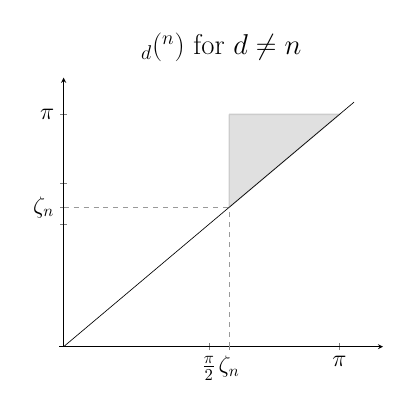
\begin{tikzpicture}[scale=0.6]
		\begin{axis} [
			title = {\LARGE $\barc\rH_d(\bS^n)$ for $d \neq n$},
			ticklabel style = {font=\Large},
			axis y line=middle,
			axis x line=middle,
			ytick={0.5,0.57,0.67,0.95},
			yticklabels={,$\zeta_n$,,$\pi$},
			xtick={0.5,0.57,0.95},
			xticklabels={$\frac{\pi}{2}$,$\zeta_n$, $\pi$},
			xmin=-0.015, xmax=1.1,
			ymin=0, ymax=1.1,]
			\addplot [thick,color=black!20!white,fill=black!30!white,
			fill opacity=0.4]coordinates {
				(0.57,0.95)
				(0.57,0.57)
				(0.95,0.95)
				(0.57,0.95)};
			\addplot [black!40!white,mark=none,dashed, thin] coordinates {(0,0.57) (0.57,0.57)};
			\addplot [black!40!white,mark=none,dashed, thin] coordinates {(0.57,0) (0.57,0.57)};
			\addplot [mark=none] coordinates {(0,0) (1,1)};
		\end{axis}
	\end{tikzpicture}
\end{tabular}
% 		\caption{Persistent homology barcode of $\bS^n$. The right-hand-side figure
% 		\emph{Right:} $\theta$-barcodes of $\VS$ where $\theta \in \cO(\ell,m)$ is any linear cohomology operation with \(\ell \neq m\).
%         In each figure, the gray region represents where additional bars could exist within the corresponding barcode.
% 		We remark that for any \(n \in \N\) the value \(\zeta_n\) is bounded below by \(\pi/2\).}
% 		\label{fig:Sk}
% 	\end{figure}


    %It is shown in \cite[Corollary 4.3]{adamaszek2018metric} that the actions of $\rC_2$ on both $\bS^{n}$ and $\bS^{n+1}$ are $r^*$-diameter actions.
    %Thus, for any $g\in \rC_2$ and $x,x'\in \bS^{n}$ such that $d(x,x') < r$, we have 
 %    Take any $y = \big[\sum \lambda_i x_i\big] \in \VR_r(\bS^{n})_G$.
 %    We have 
	% \begin{center}
	% 	$(\iota \circ \rho^{n-1})(y)
	% 	=\iota(f^{n-1}_G([\sum \lambda_i x_i]))
	% 	=\iota([f^{n-1}(\sum \lambda_i x_i)])
	% 	=[\pi^{n-1}(\sum \lambda_i x_i)]
	% 	$
	% \end{center}
	% as an element in $\bS^n_G$, and
	% \begin{center}
	% 	$(\rho^{n} \circ \iota_t)(y) = \rho^{n}(y) = f^{n}_G([\sum \lambda_i x_i]) = [f^{n}(\sum_{i=1}^k \lambda_i x_i)] = [\pi^{n}(\sum \lambda_i x_i)].
	% 	$
	% \end{center}
	% Because $\pi^{n}$ restricted to $\bS^{n-1}_G$ is equal to $\pi^{n-1}$, we conclude that $(\iota \circ \rho^{n-1})(y) = (\rho^n \circ \iota_t)(y)$ for any $y$.
	% Thus, the diagram commutes.\anibal{Please use `big' for parenthesis that are nested.}


 \medskip\lemma
If $\beta_\degp < \tfrac{\zeta_n}{2}+\zeta_\degp$, then
$\max\{|\zeta_\degp  - \beta_\degp |, \tfrac{\pi - \zeta_n}{2}\} \leq \tfrac{\zeta_n}{2}$.

Moreover, if $\beta_\degp \leq \tfrac{\pi - \zeta_n}{2} + \zeta_\degp (< \tfrac{\zeta_n}{2}+\zeta_\degp)$, then $\max\{|\zeta_\degp  - \beta_\degp |, \tfrac{\pi - \zeta_n}{2}\} = \tfrac{\pi - \zeta_n}{2}$.

\begin{proof}
    	Since $\beta_\degp \leq \tfrac{\zeta_n}{2} + \zeta_\degp$, we have
    	\[
    	\max\{|\zeta_\degp  - \beta_\degp |, \tfrac{\pi - \zeta_n}{2}\}
    	= \max\{\beta_\degp - \zeta_\degp, \tfrac{\pi - \zeta_n}{2}\}
    	< \max\{\tfrac{\zeta_n}{2}+\zeta_\degp - \zeta_\degp, \tfrac{\pi - \zeta_n}{2}\}
    	= \tfrac{\zeta_n}{2} .
    	\]
     
    	If, in addition, $\beta_\degp \leq \tfrac{\pi - \zeta_n}{2} + \zeta_\degp$, we divide the discussion to two cases.
    	When $\beta_\degp \leq \zeta_\degp$, it follows from $\tfrac{\pi}{2} < \alpha \leq \beta_\degp \leq \zeta_\degp  \leq \tfrac{2\pi}{3}$ and $\zeta_n \leq \tfrac{2\pi}{3}$ that
    	\[
    	|\zeta_\degp  - \beta_\degp |
    	= \zeta_\degp  - \beta_\degp
    	< \tfrac{2\pi}{3} - \tfrac{\pi}{2}
    	= \tfrac{\pi}{6}
    	\leq \tfrac{\pi - \zeta_n}{2}.
    	\]
    	When $\beta_\degp > \zeta_\degp$, 
    	\[
    	|\zeta_\degp  - \beta_\degp |
    	= \beta_\degp - \zeta_\degp
    	\leq \tfrac{\pi - \zeta_n}{2} + \zeta_\degp - \zeta_\degp
    	= \tfrac{\pi - \zeta_n}{2}.
    	\]
    	Thus, $\max\{|\zeta_\degp  - \beta_\degp |, \tfrac{\pi - \zeta_n}{2}\} = \tfrac{\pi - \zeta_n}{2}.$
\end{proof}


% \subsubsection{}
% \label{ss:proof of genberal_distance_comparison}
% We prove \cref{ss:genberal_distance_comparison} by combining results from \cref{subsub:db_upper_bound}, \cref{subsub:db_theta_lower_bound} and \cref{subsub:comparison_lemma}, we deduce that the lower bound of the bottleneck distance $\db$ between the $\theta$-barcodes of the two space $\VS$ and $\cX$ (Equation (\ref{eq:db_theta_lower_bound})) is larger than the upper bound of $\db$ between the persistent homology barcodes of the two spaces (Equation (\ref{eq:db_usual_upper_bound})).

% \begin{proof}[Proof of \cref{ss:genberal_distance_comparison}]
%     Let $\beta_m = 2\firstdeath{m}{\cX}$ and $\gamma_\theta = 2\firstdeath{\theta}{\cX}$.
%     By \cref{eq:db_usual_upper_bound} and \cref{eq:db_theta_lower_bound}, it suffices to show that
%     \[
%     \min\big\{\tfrac{\gamma_\theta}{2}, \zeta_n\big\} \geq \max\big\{|\zeta_m - \beta_m|, \tfrac{\pi - \zeta_n}{2}\big\}.
%     \]
%     Since \(\zeta_n \leq \crit(\cX) \leq \gamma_\theta\), we have
%     \(
%     \min\big\{\tfrac{\gamma_\theta}{2}, \zeta_n\big\} \geq \tfrac{\zeta_n}{2}.
%     \)
%     On the other hand, because \(\zeta_n \leq \crit(\cX) \leq \beta_m < \tfrac{\zeta_n}{2} + \zeta_m\), applying Part (1) of the lemma in \cref{subsub:comparison_lemma} gives
%     \(
%     \max\big\{|\zeta_m - \beta_m|, \tfrac{\pi - \zeta_n}{2}\big\} \leq \tfrac{\zeta_n}{2}.
%     \)
%     Thus, we have the desired inequality.
% \end{proof}